%------------------------------------------------------------------%
% Cannabis Data Science Presentation 10/27/2021
%
% FIXME: Add bibliography
% https://tex.stackexchange.com/questions/148893/package-biblatex-error-incompatible-package-ucs-begindocument?noredirect=1&lq=1
% https://tex.stackexchange.com/questions/261595/how-to-rerun-biber-on-the-file
% https://tex.stackexchange.com/questions/229638/package-biblatex-warning-babel-polyglossia-detected-but-csquotes-missing
% https://tex.stackexchange.com/questions/49610/use-biblatex-and-utf8
% https://stackoverflow.com/questions/1507672/putting-citation-text-on-same-slide-with-latex-beamer
%------------------------------------------------------------------%
\documentclass[xcolor={dvipsnames}]{beamer}
\hypersetup{pdfpagemode=FullScreen}
\mode<presentation> %TEMPLATE
{ \usetheme{Boadilla}
  \usecolortheme{orchid}
  \usefonttheme{default}
  \setbeamertemplate{navigation symbols}{}
  \setbeamertemplate{caption}[numbered]} 
\usepackage[english]{babel}
\usepackage[utf8x]{inputenc}
\setbeamersize{text margin left=0.5in,text margin right=0.5in}

\usepackage[dvipsnames]{xcolor}
\definecolor{DarkGreen}{RGB}{2, 48, 32}
\definecolor{CalyxGreen}{RGB}{34, 153, 84}
\definecolor{DarkOrange}{RGB}{199, 0, 57}
\definecolor{LightOrange}{RGB}{255, 87, 51}
\definecolor{LightGreen}{RGB}{218, 247, 166}
\definecolor{LightYellow}{RGB}{255, 195, 0}

\setbeamercolor*{palette primary}{bg=LightGreen, fg = DarkGreen}
\setbeamercolor*{palette secondary}{bg=LightGreen, fg=DarkGreen}
\setbeamercolor*{palette tertiary}{bg=LightGreen, fg = DarkGreen}
%\setbeamercolor*{palette quaternary}{bg=myNewColorD, fg = green}

% Margins
%\addtobeamertemplate{frametitle}{}{\vspace{-1em}}
%\setbeamersize{text margin right=5cm}

%------------------------------------------------------------------%
% FIXME: Bibliography
%------------------------------------------------------------------%
%\usepackage{csquotes}
%\usepackage[style=verbose]{biblatex}
%\addbibressource{presentation-bib.bib}

%------------------------------------------------------------------%
% Packages
%------------------------------------------------------------------%
\usepackage{amsmath}
\renewcommand*\footnoterule{} %No sperating line on footnote
\usepackage{mathtools} %ANNOTATING EQUATIONS
\usepackage{hhline} %DOUBLBARS
\newcommand\T{\rule{0pt}{2.5ex}} %TOPSTRUT
\newcommand\B{\rule[-1.25ex]{0pt}{0pt}} %BOTTOMSTRUT
\newenvironment<>{varblock}[2][.9\textwidth] %RESIZED BLOCKS
  {\setlength{\textwidth}{#1}
  \begin{actionenv}#3
    \def\insertblocktitle{#2}\par
    \usebeamertemplate{block begin}}
  {\par\usebeamertemplate{block end}
  \end{actionenv}}
\defbeamertemplate{enumerate item}{largeball} %LARGE BALLS
{\begin{pgfpicture}{-1ex}{-0.65ex}{1.5ex}{1.5ex}
\usebeamercolor[fg]{item projected}
{\pgftransformscale{2.5}\pgftext{\Large\pgfuseshading{bigsphere}}}
{\pgftransformshift{\pgfpoint{0pt}{0.5pt}}
\pgftext{\usebeamerfont*{item projected}\small\insertenumlabel}}
\end{pgfpicture}}
\usepackage{tikz} % FANCY ARROWS
\usepackage{xparse}
\NewDocumentCommand\UpArrow{O{2.0ex} O{black}}{%
   \mathrel{\tikz[baseline] \draw [->, line width=0.5pt, #2] (0,0) -- ++(0,#1);}} % FANCY UPARROW
\NewDocumentCommand\DownArrow{O{2.0ex} O{black}}{%
   \mathrel{\tikz[baseline] \draw [<-, line width=0.5pt, #2] (0,0) -- ++(0,#1);}} % FANCY DOWNARROW
%\vskip 1cm
\makeatletter
\newcommand{\LeftEqNo}{\let\veqno\@@leqno}%LEFT EQUATION #'s
\makeatother

%------------------------------------------------------------------%
% Title
%------------------------------------------------------------------%
\title[Meetup]{}
\author{Cannabis Data Science}
\institute[]{\Large Meetup}
\date{October 27, 2021}
\begin{document}
\begin{frame}{}
  
\includegraphics[scale=0.075]{images/logos/cannlytics_logo_with_text_light.png}
  \titlepage
\end{frame}

%------------------------------------------------------------------%
% Introduction
%------------------------------------------------------------------%

\section{Introduction}

%----------
% Inflation

\begin{frame}{}

{\large Cannabis Prices in Oregon}\vspace{\baselineskip}\\

\begin{center}
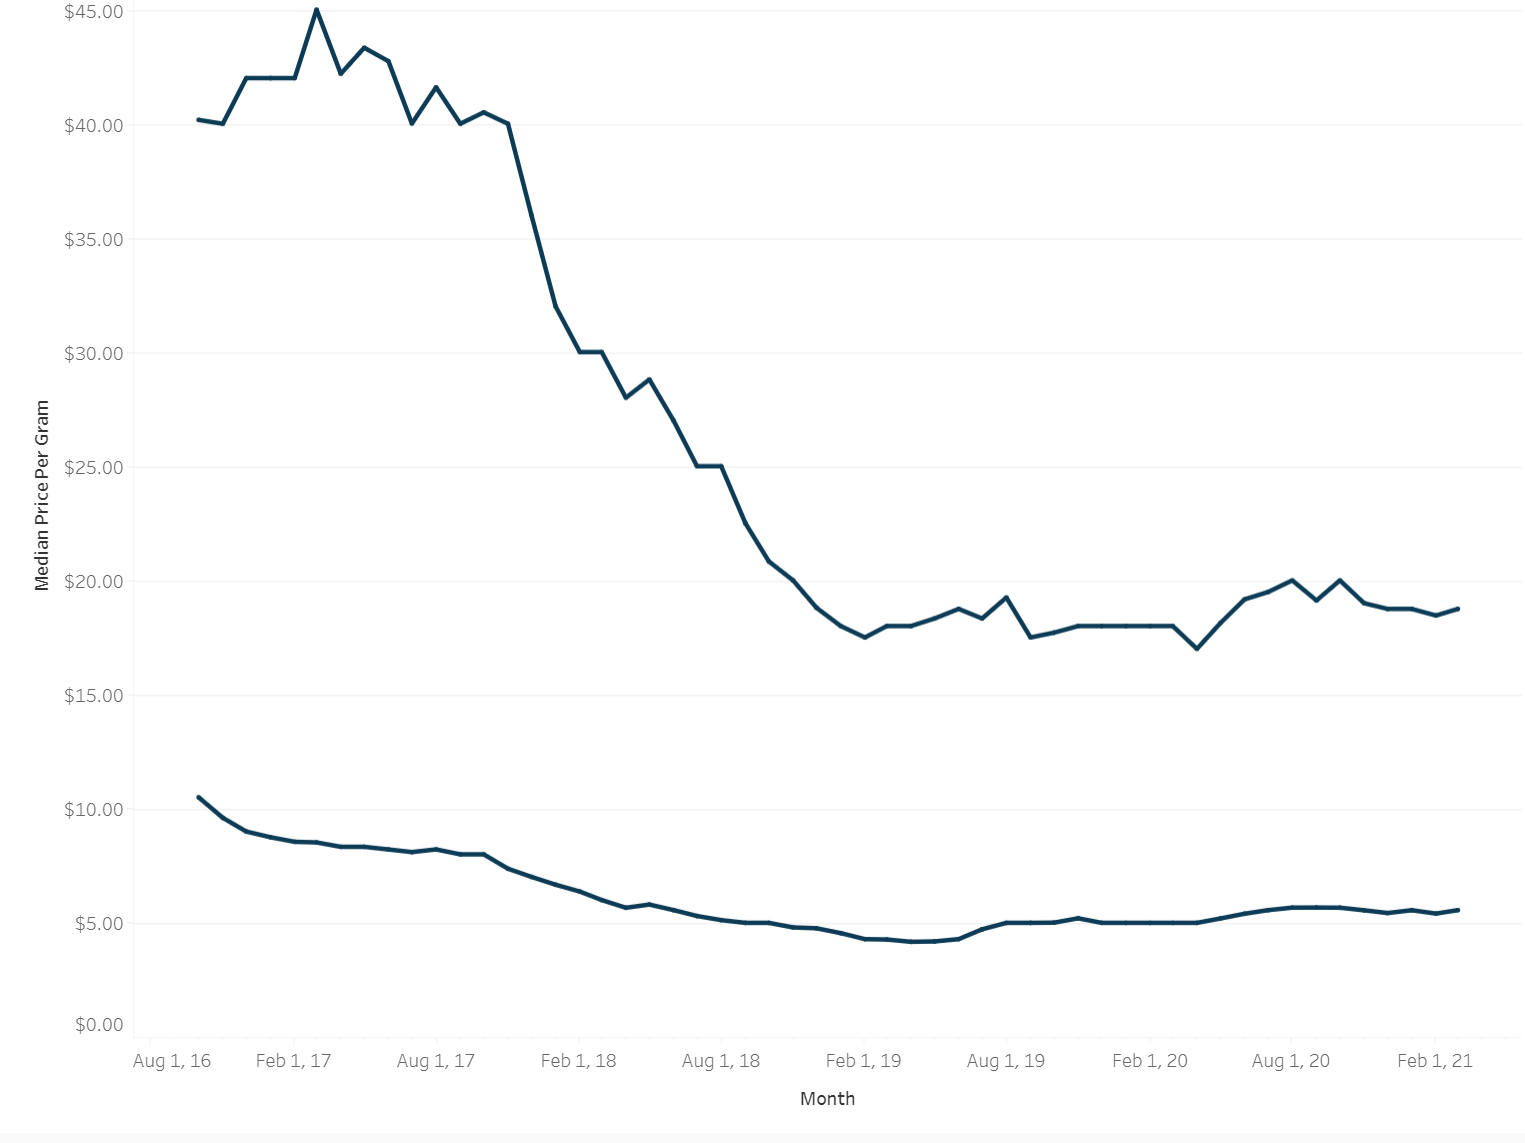
\includegraphics[width=.75\textwidth]{images/oregon-prices.png}
\end{center}

\vspace{.75\baselineskip}

\begin{block}{}
Define \textbf{inflation} as $\pi_t \equiv \frac{p_t - p_{t-1}}{p_{t-1}}$.
\end{block}

{\tiny Source: https://data.olcc.state.or.us/t/OLCCPublic/views/MarketDataTableau/Prices}

\end{frame}


%--------------
% Interest Rate

\begin{frame}{}

{\Large Interest Rates}\vspace{\baselineskip}\\

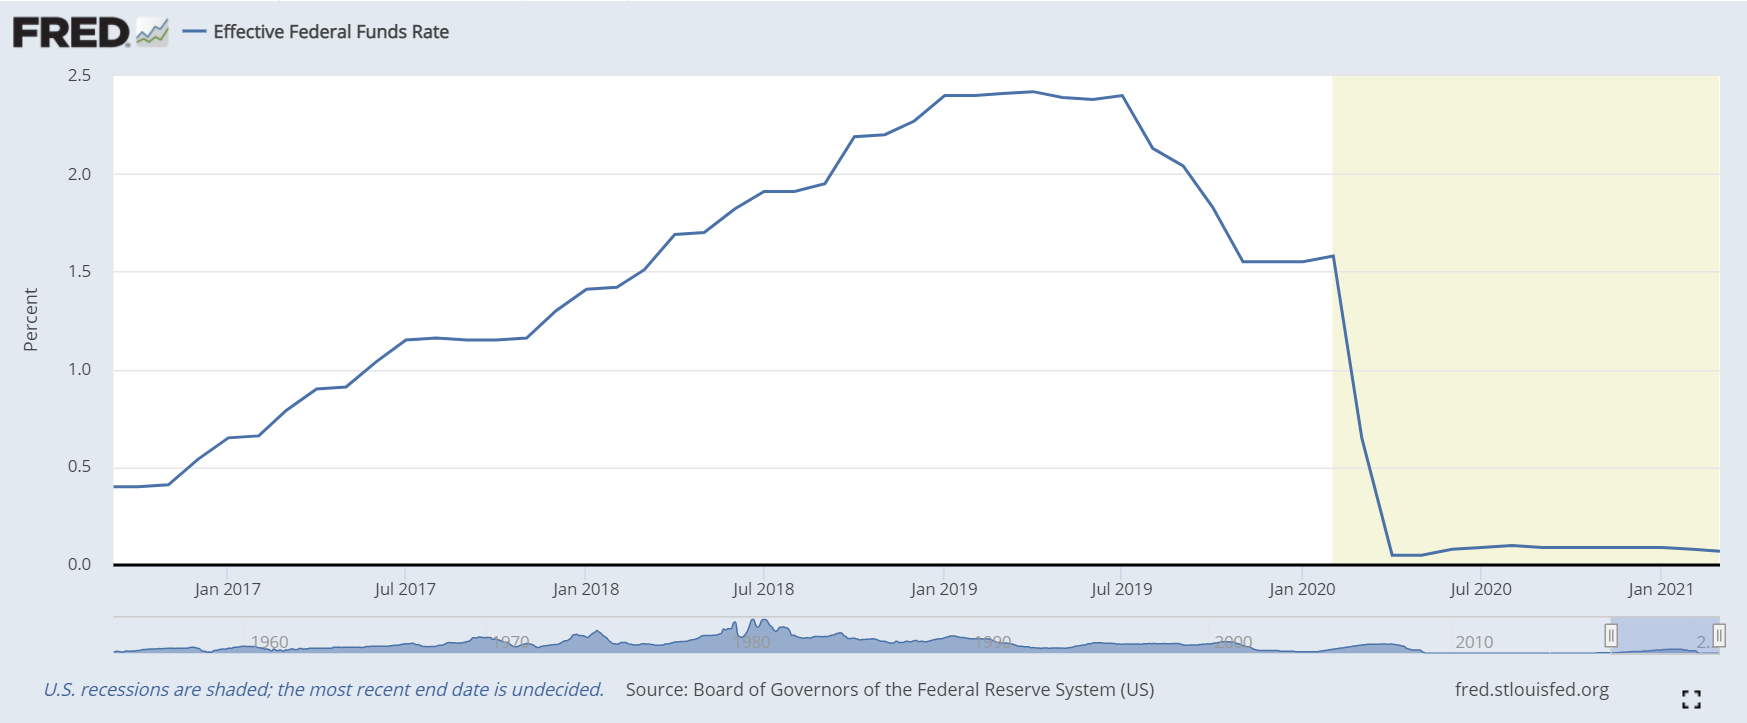
\includegraphics[width=\textwidth]{images/interest-rate.png}

\vspace{1\baselineskip}

The central bank sets policy to influence the nominal interest rate, $i_t$, as a function of
the realized output gap, $x_t$, and the rate of inflation, $\pi_t$.

\begin{block}{}
Define the \textbf{output gap} as $x_t \equiv \hat{y}_t - y_{t}$, where $\hat{y}_t$ are prior expectations for output.
\end{block}
\end{frame}


\section{Theory}

% System of equations

\begin{frame}{}

{\Large VAR Models}\vspace{\baselineskip}\\

Assume the following system of linear equations for output, $y$, inflation, $\pi$, and the interest rate, $i$.
\begin{align*}
y_t &= \alpha_ y + \dots + \beta_j y_{t-j} + \dots + \gamma_j\pi_{t-j}+\dots+\delta_j i_{t-j} + \mu_{t}^y \\
\pi_t &= \alpha_\pi + \dots + \theta_j y_{t-j} + \dots + \phi_j\pi_{t-j}+\dots+\lambda_j i_{t-j} + \mu_{t}^\pi \\
i_t &= \alpha_i + \dots + \psi_j y_{t-j} + \dots + \kappa_j\pi_{t-j}+\dots+\rho_j i_{t-j} + \mu_{t}^i
\end{align*}

\end{frame}

\begin{frame}{}

{\Large VAR Models}\vspace{\baselineskip}\\

The advantages to VAR models are that they are;

\begin{itemize}
\item Atheoretical
\item Flexible,
\item Can fit any frequency data
\end{itemize}

\vspace{1\baselineskip}

The major pitfall to VAR models is \textbf{overfitting} the model with regressors.

\end{frame}

% Policy Decisions


% Output Gap / Rational Expectations

\begin{frame}{}

{\Large VAR Model in Matrix Form}\vspace{\baselineskip}\\

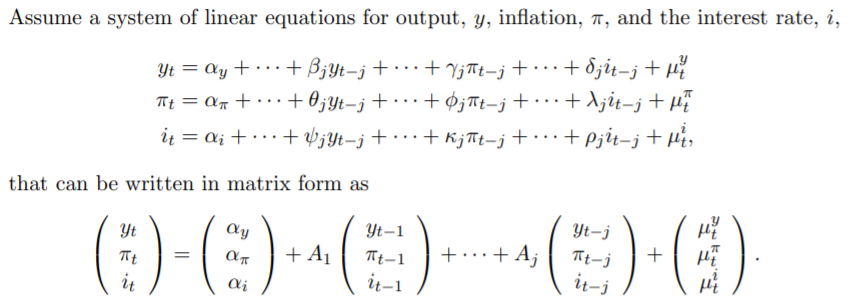
\includegraphics[width=\textwidth]{images/var_matrix_form.png}

\end{frame}

\begin{frame}{}

{\Large Forecast Model}\vspace{\baselineskip}\\

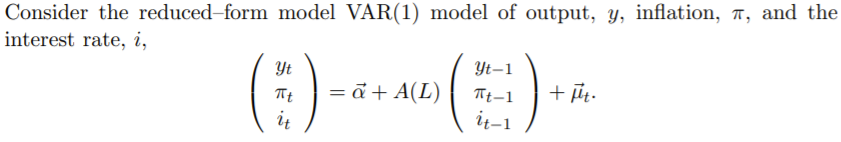
\includegraphics[width=\textwidth]{images/forecast_model.png}

\vspace{1\baselineskip}

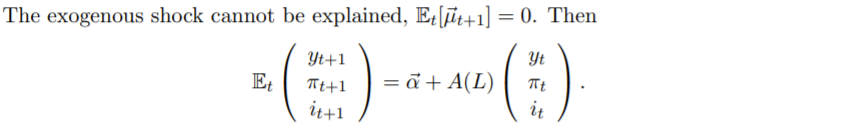
\includegraphics[width=\textwidth]{images/forecast_model_estimation.png}
\end{frame}


% Rules of Forecasting

\begin{frame}{}

{\Large The 10 Commandments of Forecasting}\vspace{\baselineskip}\\

\begin{enumerate}
\item Know what you are forecasting.
\item Understand the purpose of forecasting.
\item Acknowledge the cost of the forecast error.
\item Rationalize the forecast horizon.
\item Understand the choice of variables.
%\end{enumerate}
%\end{frame}
%\begin{frame}{}
%\begin{enumerate}
%\setcounter{enumi}{5}
\item Rationalize the forecasting model used.
\item Know how to present the results.
\item Know how to decipher the forecast results.
\item Use recursive methods.
\item Understand that forecasting models evolve over time.
\end{enumerate}
\end{frame}

% RMSE

%\begin{frame}{}
%The out-of-sample root mean square error (RMSE) can quantify forecast error.
%
%$$
%RMSE = \sqrt{\frac{1}{T}\Sigma(Y_{t+1} - \hat{Y}_{t+1})^2}
%$$
%\end{frame}

\section{Application}

% Forecasting steps

% 1.
%\begin{frame}{}
%{\Large 1. Know what you are forecasting}\vspace{\baselineskip}\\
%\begin{itemize}
%\item We are simultaneously forecasting output, $y$, inflation, $\pi$, and the federal funds rate, $i$, for the remainder of the year.
%\end{itemize}
%\end{frame}
%
%% 2.
%\begin{frame}{2. Understand the purpose of forecasting}
%{\Large }\vspace{\baselineskip}\\
%\begin{itemize}
%\item Get better expectations for the size of the Colorado cannabis industry in 2021.
%\end{itemize}
%\end{frame}
%
%% 3.
%\begin{frame}{3. Acknowledge the cost of the forecast error.}
%{\Large }\vspace{\baselineskip}\\
%\begin{itemize}
%\item Overstating growth may lead to foolhardy decisions, where as understating growth may leave money on the table.
%\end{itemize}
%\end{frame}
%
%% 4.
%\begin{frame}{4. Rationalize the forecast horizon}
%{\Large }\vspace{\baselineskip}\\
%\begin{itemize}
%\item Forecasting a series for 2021 is a long, yet informative horizon. A shorter time frame may be less informative and a longer time frame may yield unreliable forecasts.
%\end{itemize}
%\end{frame}
%
%% 5.
%\begin{frame}{5. Understand the choice of variables.}
%{\Large }\vspace{\baselineskip}\\
%\begin{itemize}
%\item Historic plant totals and cannabis sales in Colorado from January 2014 through June 2020 will be used, utilizing all of the available data under the principle to never throw away data.
%\end{itemize}
%\end{frame}
%
%% 6.
%\begin{frame}{6. Rationalize the forecasting model used.}
%{\Large }\vspace{\baselineskip}\\
%\begin{itemize}
%\item A atheoretical forecasting approach, Box-Jenkins methodology, will be utilized.
%
%The advantages to VAR models are that they are atheoretical, flexible, and can fit any frequency data. The major pitfall to VAR models is overfitting the model with regressors.
%
%\vspace{\baselineskip}
%AR(p) process:
%$$
%y_t = \alpha + \beta_1 y_{t-1} + \beta_2 y_{t-2} + ... + \beta_p y_{t-p} + \epsilon_t
%$$
%MA(q) process:
%$$
%y_t = \theta + \gamma_1 \epsilon_{t-1} + \gamma_2 \epsilon_{t-2} + ... + \gamma_q \epsilon_{t-q} + \epsilon_t
%$$
%\end{itemize}
%\end{frame}
%
%% 7.
%\begin{frame}{7. Know how to present the results.}
%{\Large }\vspace{\baselineskip}\\
%\begin{itemize}
%\item Always show the data (in this case in a figure).
%\end{itemize}
%\end{frame}
%
%% 8.
%\begin{frame}{8. Know how to decipher the forecast results.}
%{\Large }\vspace{\baselineskip}\\
%\begin{itemize}
%\item Look for seasonality, etc.
%\end{itemize}
%\end{frame}
%
%% 9.
%\begin{frame}{9. Use recursive methods.}
%{\Large }\vspace{\baselineskip}\\
%\begin{itemize}
%\item When future data is released, calculate the RMSE for actual forecasts and create new forecasts.
%\end{itemize}
%\end{frame}
%
%% 10.
%\begin{frame}{10. Understand that forecasting models evolve over time.}
%{\Large }\vspace{\baselineskip}\\
%\begin{itemize}
%\item See if better forecasting models predict better.
%\end{itemize}
%\end{frame}


%------------------------------------------------------------------%
% Takeaway
%------------------------------------------------------------------%

\begin{frame}{}

{\Large Alternative Models}\vspace{\baselineskip}\\

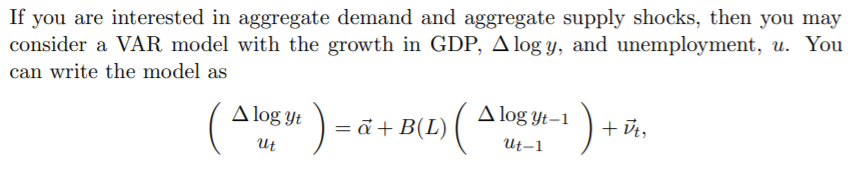
\includegraphics[width=\textwidth]{images/aggregate_demand_model.png}

\vspace{1\baselineskip}

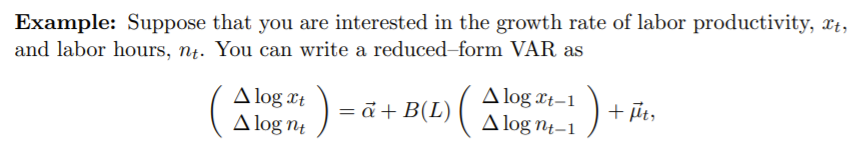
\includegraphics[width=\textwidth]{images/labor_productivity_model.png}
\end{frame}


\begin{frame}{}
\begin{center}
\begin{minipage}{3.85in}
\begin{block}{Until next time}
Make some forecasts and next week we can check our forecasts.
\end{block}

\end{minipage}
\end{center}
\end{frame}

%------------------------------------------------------------------%
\end{document}
%------------------------------------------------------------------%
